\documentclass[12pt]{article}

\usepackage[backend=bibtex]{biblatex}
\addbibresource{bibliography}

\usepackage{multicol}

\usepackage{amsfonts}
\usepackage{amsmath}

\usepackage{xcolor}
\usepackage{listings}

\usepackage{graphicx}
\graphicspath{ {./images/} }

\usepackage{nameref}

\usepackage{lscape}

\definecolor{mGreen}{rgb}{0,0.6,0}
\definecolor{mGray}{rgb}{0.5,0.5,0.5}
\definecolor{mPurple}{rgb}{0.58,0,0.82}
\definecolor{backgroundColour}{rgb}{0.95,0.95,0.92}

\lstdefinestyle{CStyle}{
	backgroundcolor=\color{backgroundColour},   
	commentstyle=\color{mGreen},
	keywordstyle=\color{magenta},
	numberstyle=\tiny\color{mGray},
	stringstyle=\color{mPurple},
	basicstyle=\footnotesize,
	breakatwhitespace=false,         
	breaklines=true,                 
	captionpos=b,                    
	keepspaces=true,                 
	numbers=left,                    
	numbersep=5pt,                  
	showspaces=false,                
	showstringspaces=false,
	showtabs=false,                  
	tabsize=2,
	language=C
}

\title{Reachability analysis for continuous one-counter automata}
\author{Lars Van Roy\\
\textit{dept. of Mathematics and Computer Science} \\
\textit{University of Antwerp}\\
lars.vanroy@student.uantwerpen.be}

\begin{document}
\maketitle{}

\begin{abstract}
\noindent
Reachability is a known problem that can heavily affect the efficiency of code. It has been proven that reachability is decidable for continuous one counter timed automata which we will utilise in our approach. The proposed approach will provide a means to convert c code to one counter timed automata followed by an algorithm which is capable of analysing the reachability of each of the nodes within the generated automata. This is an extension to existing research in which we already provided a means to perform the conversion from code to automata. Within this paper, this approach will be repeated here, as the approach is specifically intended to be combined with this predecessor. Finally, we will apply the combination of approaches on an existing code base, as to determine the usefulness of the approach.

\end{abstract}

\section{Introduction}
A well known problem in writing code is the reachability of specific lines in said written code. It is often impossible to properly determine whether or not a line of code guarded by a conditional statement is going to be reachable in any possible execution of the code \cite{713323, 10.1145/1292316.1292319}. Unreachable code is never desired, but is an ever more pressing issue for energy restrained environments such as embedded computer systems \cite{embeddedefficiency}. In these systems, we want our execution to be as efficient as possible, and therefore avoid conditions that can never be satisfied or lines that can never be reached. to remedy this, a proper reachability prevention approach is needed.

To analyse the reachability, we will make use of the fact that code is quit easily convertible to automata. All statements within the code that are related to counter updates can directly be converted to operations within an automaton. Each line of code can represented by one or more nodes and a traversal of an automaton can be directly linked to the traversal of the code itself.

The continuous one counter automata are especially interesting as it has been proven that reachability is decidable for this type of automata \cite{succintandparametriconecounter, danialandjoel, blondin2021continuous}. In this paper we will provide a practical implementation for the theoretical approach that was provided by Tim Leys et al.\cite{blondin2021continuous} which can be used to prove reachability of nodes. 

Adding the restriction of only allowing a single parametric clock has a big effect on the types of code we can analyse. However, this is unavoidable, since there is no proof for two counter machines. Three counter machines and up have been proven to be undecidable \cite{FEARNLEY201526}.

In this paper we will provide the overview of an approach which will convert c code to a one counter automaton. Using the result of this first step, we will then provide a means to analyse the reachability of any of the nodes of said automaton. The following steps are taken without our approach to prove the existence of dead code.

\begin{enumerate}
	\item Convert c code into a parse tree, using ANTLR
	\item Perform context free reductions on this parse tree
	\item Perform context sensitive reductions on this parse tree
	\item Validate the resulting parse tree, to be conforming to the code constraints
	\item Generate the counter automaton
	\item Analyse which nodes are reachable
	\item Link potential unreachable statements back to the lines within the original code base
\end{enumerate}

The code can at most contain one counter and for the continuation of this paper we will only consider examples where this holds. Cases with no counter will not be considered as these are assumed to be trivial. Furthermore, the operations on the counter will be restricted, the counter can only be updated via assignments with parameters or constants, and the counter can only be compared using equality, inequality, strict less than, strict greater than, less than or equal, greater than or equal, and only to parameters or constants. As a final code constraint, the function parameters are not allowed to be altered throughout the duration of the code.

Other then the described code constraint, functions must also have a boolean return type, and integer parameter types (if any) to be converted into a counter automaton.

\section{Motivation}
Popular IDE's do already implement reachability analysis up to a certain degree. However, the dead code elimination they perform is shallow and limited. The code example given below was executed using Clion, one of the more commonly used C IDE's. While it is known that Clion can find dead code that directly results from code, it was not able to resolve this case, where the condition on line 4 can never evaluate to true. This is because the for statement on line 3 will always prevent line 4 from evaluating to true and yet Clion did not detect this. 

\begin{lstlisting}[style=CStyle]
bool is_mul(int a, int b) {
  int temp = b;
  for(; temp > 0;){
    if(temp == 0){
      break;
    }
    temp -= a;
  }
  return temp == 0;
}

int main() {
  printf("5 is a multiple of 2: %d\n", is_mul(2, 5));
  printf("6 is a multiple of 2: %d\n", is_mul(2, 6));
}
\end{lstlisting}

The approach provided within this paper will be able to detect this, as it can simply evaluate the possible values with which line 5 can be reached, it will result that there is no sequence in which line 5 can be reached and we can therefore conclude that the condition surrounding this statement can never be satisfied.

The impact of removing this line can be significant if considering cases where bigger numbers are passed. In those cases the loop on line 3 will be executed several times, making the condition on line 4 being quit impactful on the total evaluation time of this function. This clearly shows that there is value in enhanced dead code elimination, compared to the current standards. 

\section{Preliminaries}
This paper will make use of counter automata and more specifically one counter automata. These automata are derived from the general definition of automata and signify an extension by adding the notion of counters.

\subsection{General automata}
The automata used in this research are a specific subset of the generally defined automata. The general definition for an automaton A is given by the tuple (Q, $\Sigma$, $\delta$, $q_0$, F) where
\begin{itemize}
	\item Q is the set of states
	\item $\Sigma$ is a finite set of symbols, called the alphabet of the automaton
	\item $\delta: Q \times \Sigma \rightarrow Q$ is the transition function
	\item $q_0 \in Q$ is the initial state
	\item $F \subseteq Q$ is a set of states of Q defining the final states, 
\end{itemize}

\subsection{Parametric counter automata}

A one-counter automaton is a tuple $\mathcal{A}$ = $(Q, q_0, \sigma, op, F)$ where
\begin{itemize}
	\item $Q$ is a finite set of states
	\item $q_0 \in Q$ is the initial state
	\item $F \subseteq Q$ is the set of accepting states
	\item $op$ is the set of operations
	\item $\sigma \subseteq Q \times op \times Q$ is the transition relation with $op$ the set of operations
\end{itemize}

The counter valuation $c \in \mathbb{N}$ is the value that will be analysed and updated during the evaluation of the automaton.

At all times the automaton will be in a configuration $(q, c)$ where $q \in Q$ and $c$ the counter valuation where $(q_0, 0)$ is the initial configuration.

Parametric counter automata, as compared to regular counter automata, allow counters to be modified by parameters as well as constants. As the counters need to be integers, we will only allow integer type paramters. We will consider the following set of allowed operations where $P$ is the set of parameters, the $\epsilon$ symbol will be used to represent an empty label.
\[
 op = \{+c, -c, +p, -p, \leq c, =c, \geq c, \leq p, =p, \geq p: c \in \mathbb{N}, p \in P\} \cup \{\epsilon\}
\]

The automata we will consider will be one-counter parametric automata. The set $Q$ will contain a state for each line of code. The initial state $q_0$ will be the state corresponding with the first line of code. For now the set of final states $F$ will be empty, but the intended interpretation of a final state will be the line of which the reachability will be checked. The transition relation will consist of elements of the form $(q_i, l, q_{i+1})$ where $q_i, q_{i+1} \in Q$ and $l \in op$. 

There are a few exceptions to the above described states, some segments will have additional nodes to avoid confusion. These special nodes, and their meaning, will be further explained in their relevant sections inside Section \ref{sec:generation}, \nameref{sec:generation}.

\section{Program}
The program that will perform the conversion from c code to a one counter automaton, will do this in five steps.

The first step, the initialization, will simply generate a parse tree, using the default c grammar, with the addition of the boolean type, and the removal of some gcc extensions.

The second step, the context-free abstract syntax tree generation, will generate an abstract syntax tree without any regard for neighboring nodes.

In the third step, the abstract syntax tree generated in the previous step will be simplified in a context-sensitive manner, which means that the program will now look at all neighboring nodes. All redundant nodes will be removed, so that only important nodes with unambiguous meaning remain.

The fourth step will be an analysis on whether or not the resulting abstract syntax tree conforms to all earlier specified requirements and, if this is the case, we will continue with the fifth step, which will be the generation of the counter automaton.

We will allow all counter operations that can directly be supported by the $op$ set described earlier. We will add assignment and inequality to this, as these can easily be represented as sequences of operations in the $op$ list. Along with these we will also need support for strict less than and greater than, which can also be implemented using the operations in the \textit{op} list. The full explanation on how this can be done, can be found in Section \ref{sec:generation}.

\subsection{Initialization}
The program will start of by running the generator ANTLR compilation unit on the given c code. In case there are any issues regarding simple compilation rules, the program will exit with an error, indicating the issues in the code. For the remainder of the execution, the code is assumed to be correct, and there will be no regard for potential issues within the code.

\subsection{Context-free abstract syntax tree generation}
Using the parse tree resulting from the ANTLR compilation, we will try to generate an abstract syntax tree that is as simple as possible without regarding any context. 

First of all, the code uses the notion of a node stack. This node stack will be used to store the nodes that are currently being evaluated.

The first loop will operate as a visitor, which will traverse the parse tree in a depth first manner. The first discovery of a node is done by calling the enter function corresponding to the type of node. As soon as all children of said node have been evaluated, the corresponding exit function will be called. 

However, the creation of nodes is not the same in all situations, in some cases, a specific kind of node will be created, and in other cases a specific kind of node will not be created, depending on the rule used for the current node (which we can determine from the context of the current node). In order to know whether or not we need to pop a node from the node stack, we will allow the code to look at the top node in the stack, and evaluate the type of set node. No other context related evaluations will be allowed.

\subsubsection{Context-free analysis assignmentExpression example}
To look at a concrete example, consider the following rule in the grammar:
\begin{align*}
	&assignmentExpression\\
	&\text{:}\indent \text{conditionalExpression}\\
	&|\indent \text{unaryExpression assignmentOperator assignmentExpression}\\
	&|\indent \text{Digitsequence}; \\
\end{align*}
The rule for conditionalExpression needs to be there, as there is a chain of expressions, and some expressions need to be higher in the order than others, therefore all expressions with a higher priority need to be evaluated before the lower priority expressions. This is done by adding a rule to a lower priority expression in each expression class. It is however undesirable for these nodes to be added. Without regard for context in other nodes, we can simply look at the current node to see whether or not the conditionalExpression line is used (which ANTLR generated context allows us to do).

Since there is a chance no new node was added within the enter function, we will also be required to evaluate the top of the stack, to see whether or not the top of the stack is a node we need to pop, the code will do the same check that was done in the enter function of the traversal.

\subsection{Context-sensitive abstract syntax tree reduction}
There is still the need for 
 reductions. We will attempt to implement constant propagation and substitution, in which we compute constant expressions, and replace variables with known value, by their actual value. Furthermore we will try to rephrase expressions by expressions with the same meaning, so that all expressions, if possible, are in an acceptable format for the counter automaton.

The context-sensitive reduction will also keep track of a lot of data about the variables in a symbol table. It will track whether or not variables are current initialized with a known value, values at certain points within the execution, it will track struct, union and enum definitions used for folding and so on. It will keep track of the kind of variables we have (eg. counters and parameters). All of this info will be used to enable the operations this cycle will perform, but will also be used in the validation loop.

The program will do this by traversing the abstract syntax tree resulting from the previous step, but will now specifically go through the children of relevant expressions (eg. assignment expressions, additive expressions, ...).

Important to note is that no folding/substitution will occur within loops, as these operations occur a variable number of times, and since there is no way of determining the exact number of times without evaluating the expression, this is considered too complex and often impossible, as counters may depend on parameters, which need to be chosen at evaluation time.


\subsubsection{Context-sensitive reduction example: constant propagation}
Another example of a needed reduction, is constant propagation and folding. It is possible that a code segment would initially be rejected, due to use of unwanted variables, while in essence, these variables are nothing but variable representations of results of constant expressions. Consider the code snippet below. It would initially be rejected, because the counter variable is initialized with a variable that is neither a constant nor a parameter.
\newpage
\begin{lstlisting}[style=CStyle]
bool divide(int p, int n){
	int variable = 5;
	variable += 20;
	int counter = variable;
	while(counter > 0){
		counter -= n;
	}
	counter += 1;
	counter -= 1;
	if(counter == 0){
		return true;
	}
	return false;
}
\end{lstlisting}

However, due to constant propagation and folding, we can simplify the two statements on line 2 and line 3, so that they become.

\begin{lstlisting}[style=CStyle]
int variable = 25;
\end{lstlisting}

Now that the variable is just a constant, we can substitute this variable in the declaration of counter, so that we now have the following.
\begin{lstlisting}[style=CStyle]
int variable = 25;
int counter = 25;
\end{lstlisting}

The new code segment is acceptable, but we will not stop here, as the first line of the code is useless. It has no further benefit for the execution and will therefore be dropped. The final counter assignment will not be folded. Whenever a variable gets altered within a conditional scope, the variable is considered to be uncertain, and further folding based on earlier values will not be allowed. The final code segment is as described below, which is trivially accepted to be converted to a counter automaton.

\begin{lstlisting}[style=CStyle]
bool divide(int p, int n){
	int counter = 25;
	while(counter > 0){
		counter -= n;
	}
	counter += 1;
	counter -= 1;
	if(counter == 0){
		return true;
	}
	return false;
}
\end{lstlisting}

\subsubsection{Context-sensitive reduction example: addition folding}
As described earlier, we do allow additions and subtractions of the form $-x, +x, -n$ and $+n$, where $x \in P$ or $n \in \mathbb{N}$ with $P$ the set of parameters. Given that the formation, described in Figure \ref{fig:unfolded_addition} occurs in the automaton, we would technically not be allowed to accept this, as this is not directly in the specified format.

\begin{figure}[h]
	\centering
	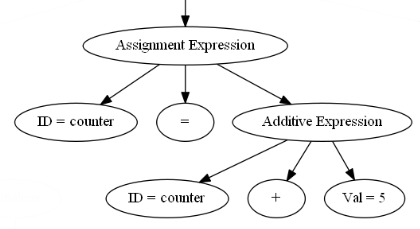
\includegraphics[width=0.8\linewidth]{unfolded_addition}
	\caption{An Assignment Expression with counter addition as value.}
	\label{fig:unfolded_addition}
\end{figure}

However, the context-sensitive reduction will be able to reduce the earlier specified example to the automaton in Figure \ref{fig:folded_addition}. This automaton will be acceptable, as this is a direct use of an allowed operation.

\begin{figure}[h]
	\centering
	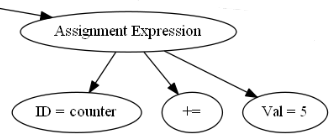
\includegraphics[width=0.6\linewidth]{folded_addition}
	\caption{An Assignment Expression with constant as value.}
	\label{fig:folded_addition}
\end{figure}
\newpage
\subsubsection{Nodes}
After the cleaning cycle has finished, there will only be a relatively small set of nodes remaining. Below a quick overview and their meaning within the syntax tree.

\begin{multicols}{2}
	\noindent
	\textbf{Compilation Unit} indicates the root of each Abstract Syntax Tree.\\
	\textbf{Function Definition} indicates the definition of a new function.\\
	\textbf{Function Specifier} indicates specifier of function.\\
	\textbf{Generic} head node for generic specification.\\
	\textbf{Generic Association} indicates a generic association.\\
	\textbf{Parameter Type List} head of the specification of all parameters of a function.\\
	\textbf{Parameter Declaration} head node of the declaration of a single parameter.\\
	\textbf{Compound Statement} indicates a scope defined by \{ \} brackets.\\
	\textbf{Type Specifier} indicates that the child(ren) of this node need to be regarded as being known type(s).\\
	\textbf{Type Name} indicates that the child(ren) of this node need to be regarded as being a type(s).\\
	\textbf{Type Def Name} indicates the definition of a type.\\
	\textbf{Declaration} indicates a declaration, this can contain multiple types and identifiers. In case of a function, the function name and parameter types plus identifiers will all belong to a single declarator node.\\
	\textbf{Init Declarator} defines a declaration of a variable with an initial value.\\
	\textbf{Direct Declarator} defines a declaration of a variable with a second variable.\\
	\textbf{Declarator} head node for the variable name part of the declaration.\\
	\textbf{Initializer} head node for the value part of the declaration.\\
	\textbf{Primary Expression} defines the most basic expression, eg. brackets, identifiers, constants, ... .\\
	\textbf{Postfix Expression} defines a postfix expression.\\
	\textbf{Unary Expression} defines a unary expression.\\
	\textbf{Cast Expression} defines a cast expression.\\
	\textbf{Multiplicative Expression} defines a multiplicative expression.\\
	\textbf{Additive Expression} defines an additive expression.\\
	\textbf{Shift Expression} defines a shift expression.\\
	\textbf{Relational Expression} defines a relational expression.\\
	\textbf{Equality Expression} defines an equality expression.\\
	\textbf{Bitwise And Expression} defines a bitwise and expression.\\
	\textbf{Bitwise Xor Expression} defines a bitwise exclusive or expression.\\
	\textbf{Bitwise Or Expression} defines a bitwise inclusive or expression.\\
	\textbf{Logical And Expression} defines a logical and expression.\\
	\textbf{Logical Or Expression} defines a logical or expression.\\
	\textbf{Conditional Expression} defines a conditional expression.\\
	\textbf{Assignment Expression} defines an assignment expression.\\
	\textbf{Expression} head node in case of multiple expressions.\\
	\textbf{For Declaration} head node for the first clause of a for loop.\\
	\textbf{For Expression} head node for a clause of a for loop.\\
	\textbf{For Condition} head node for the condition part of the second clause of a for loop.\\
	\textbf{Iteration Statement} defines an iteration statement (for, while, do while).\\
	\textbf{Jump Statement} defines a jump statement.\\
	\textbf{return} indicates return statement.\\
	\textbf{Labeled Statement} indicates a labeled statement.\\
	\textbf{Struct or Union Specifier} indicates the specification of a struct or union.\\
	\textbf{Enum Specifier} indicates the specification of an enumerator.\\
	\textbf{Struct Declaration} head node for a struct declaration.\\
	\textbf{Struct Declarator} head node for a struct declarator.\\
	\textbf{Static Assert Declaration} defines static assertion.\\
	\textbf{Enumerator} specifies variables part of an enumerator.\\
	\textbf{Size} head for array size.\\
	\textbf{Default} defines the default option for switch statement.\\
	\textbf{Alignment Specifier} defines an alignment restriction to an identifier.\\
	\textbf{Atomic Type Specifier} defines an atomic type.\\
	\textbf{Arguments} head node for arguments part of a function call.\\
	\textbf{sizeof} defines sizeof operation.\\
	\textbf{\_Alignof} defines \_alignof operation.\\
	\textbf{Val = $<$value$>$} defines a constant. \\
	\textbf{ID = $<$id$>$} defines a variable name.
\end{multicols}

\subsection{Abstract syntax tree validation}
The fourth loop will iterate over the abstract syntax tree resulting from the previous step, and while doing so, it will evaluate the nodes that occur and the context in which they occur.

The majority of the node evaluation is represented in a list of unsupported nodes. Most of these nodes are head nodes for certain kinds of expressions which will never be supported.

\begin{align*}
	unsupported = \left\{ \begin{array}{l}
		Multiplication\ Expression, sizeof, \_Alignof, \\
		\&, *, -, +, ., ->, !, ~, Cast\ Expression, \\
		Shift\ Expression, Bitwise\ And\ Expression, \\
		Bitwise\ Or\ Expression, Bitwise\ Xor\ Expression, \\
		*=, /=, \%=, <<=, >>=, \&=, ^=, |=, \\
		Logical\ And\ Expression, Logical\ Or\ Expression, \\
		Additive\ Expression
	\end{array} \right\}
\end{align*}

Whenever we encounter a node part of the $unsupported$ set, the current situation will be inspected. For example, if a \textit{Multiplication Expression} node occurs, inside a subtree of an \textit{Assignment Expression} node where an assignment to a counter was specified, we know that we are in an invalid state, as counters can only be updated via assignments, additions or subtractions. 

The same logic holds for subtrees of conditional expressions. In case we have a conditional expression where the subtree contains a \textit{Bitwise And Expression} node, we know that this is an invalid state, as constant conditions have already been folded in the previous step, this must mean that there is a counter in the condition, but counter comparisons are not allowed to contain and statements.

Furthermore, all variable usage will be tracked. We will allow multiple counters to exist, as long as we can substitute one general counter without having any conflicts, in other words, there can't be any overlap between counter usages. This is simply tracked by tracking the nodes in which the counter variables occur, with the exception of when they occur within conditional scopes. If this is the case, their first usage is set to the first line of the scope, so that overlap does occur when a different counter is used for the condition of the scope. 

Finally, the initial value will be tracked. In case there is a declaration with an initial value, this value will be chosen, otherwise it will be set to 0, which is the default integer value in C. This initial value allows us to skip over declarations in the generator. We can simply set the counter value to the initial value of the used counter at that point in time, just before its first usage.

Another aspect that will be tested, is the function definition. A function needs to have a boolean return type, and can only have integer parameters. If this not the case, an error status will be added.

These conditions will all be tracked separately for each function. Whenever the status list is empty at the end of the evaluation, we assume that no issues occurred, and we say that the function satisfies the requirements, if there are any issues, no counter automaton will be generated, and the errors will be printed to the terminal.

Important to note is that there is no regard for global statements. These are considered to be variable and undetermined. It could be that they can perfectly be used as counters, and that they will never be altered by other functions, but it is impossible to determine this efficiently. Therefore, a counter must be declared within the function scope.

\subsubsection{validation example}
When we go back to the earlier mentioned segment of code. We obtain the automaton displayed in Figure \ref{fig:divide_cleaned}.

\begin{lstlisting}[style=CStyle]
bool divide(int p, int n){
	int counter = p;
	
	while(counter > 0){
		counter -= n;
	}
	
	if(counter == 0){
		return true;
	}
	return false;
}
\end{lstlisting}

\begin{figure}[h]
	\centering
	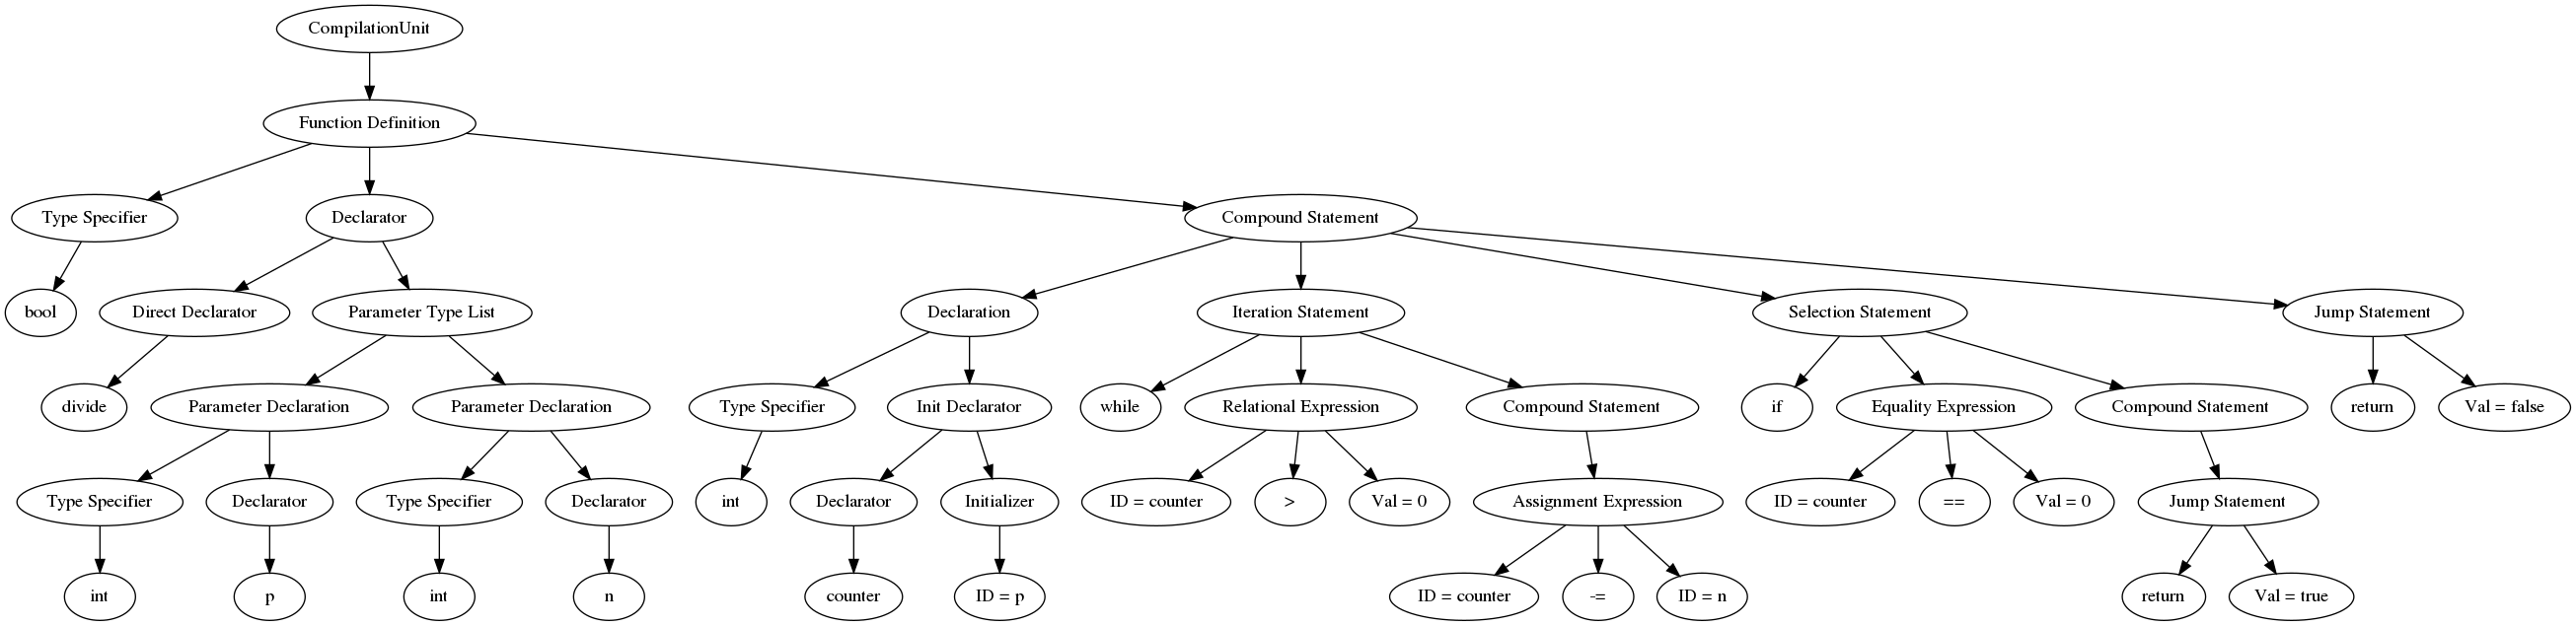
\includegraphics[width=\linewidth]{divide_cleaned}
	\caption{The cleaned Abstract Syntax Tree of the divide function.}
	\label{fig:divide_cleaned}
\end{figure}

We can immediately see that the function conforms to the required function definition, as the return type is boolean, as can be seen from the leftmost node. The parameters are also of type int, which can be seen from the parameters defined underneath the 'Parameter Type List' node.

From the cleaner we know which variables are counters, and we can see that the first declaration is a counter, but we will skip the declaration, as we know the value which is stored in the initial value, the initialization will happen before the first operation on the counter occurs. 

Next, we encounter the Iteration statement, for which we will check the condition with the constrained conditional variable enabled. With this variable enabled, we can simply continue traversing the nodes, and in case there are any unsupported nodes, the corresponding error would automatically be generated. However, there will be no corresponding nodes, so we will leave the Relational Expression without any error statuses, and we will disable the constrained conditional variable. 

Next we will enter the compound statement, which symbolizes the inner scope of the iteration statement. We will encounter an Assignment Expression with a variable that we know is a counter, we will therefore enable the counter assignment variable, while traversing the children of this node. No invalid nodes will appear, and we will disable the counter assignment variable when leaving the Assignment Expression node. 

The selection statement will be evaluated in the exact same manner as the Iteration Statement was evaluated, and as the jump statement holds no special operations, we can conclude that this function satisfies the requirements for one counter automaton generation.

\subsection{Counter automaton generation}
\label{sec:generation}
The final section of the program will be the counter generation itself. In this loop, there will be no more regards to possible invalid statements. At this point we assume everything to be known, and we can therefore simplify things drastically. Recall that the following list is the collection of allowed labels for the counter automaton.
\[
op = \{+c, -c, +p, -p, \leq c, =c, \geq c, \leq p, =p, \geq p: c \in \mathbb{N}, p \in P\} \cup \{\wedge\}
\]
This allows us to just check the head nodes related to such expressions.

\subsubsection{Functions}
First of all, we need the notion of the Function Definition statements. The generator will generate a counter automaton for each function, and needs to know when these start.

\subsubsection{Assignments}
Other than functions, we will also need to know when assignments to counters occur, so that we can add the proper transition labels. We only need to check whether or not we are assigning to a counter, if so, we read the operation used, and the variable that gets assigned. Valid counter assignments need to be of the form \textit{c op x} where $c$ is the counter, $op \in $ \textit{\{=, +=, -=\}} and $x \in P \lor x \in \mathbb{N}$. 

As mentioned earlier, assignments are not in the set of operations, but they can be represented using the operators displayed earlier, as can be seen in Figure \ref{fig:counter_assignment}. This can be done by using a reset operation, where we first check whether or not the counter is smaller or equal to the desired value. If so, it is either already satisfied, in which case we can just carry on, or it is smaller than the desired value, for which we will add a self loop with $+1$ as a label, so that we will eventually reach the desired value. 
\begin{figure}[h]
	\centering
	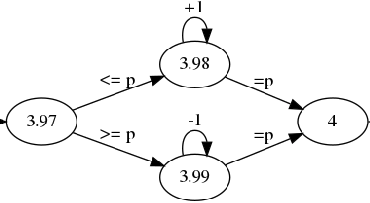
\includegraphics[width=0.48\linewidth]{counter_assignment}
	\caption{Assignment of a value p to a counter.}
	\label{fig:counter_assignment}
\end{figure}

The same thing can be done when the counter is larger or equal to the desired value, if so, it is either already satisfied, in which case we can just carry on, or it is larger than the desired value, at which point we will decrement the counter with a self loop of -1, until the condition is satisfied.

An important thing to remark, is that we are not interested in general properties of runs for these automata. We are interested in the possibility of reachability or in other words, the existence of one path that will take us to a given node. In the given example, there is a path where we would remain in node 3.98 indefinitely but since there is at least one path that would take us to node 4, node 4 is still considered reachable.

\subsubsection{Inequality conditions}
\label{sec:inequality}
Another statement we will need to support, are inequality conditions. If we want our conditional statements to be properly functioning, we will need to be able to generate opposing conditions, but the opposing condition of the equality condition, is the inequality condition, which we can not directly model using the given operations.

The following code segment makes use of an if statement which has an equality condition in it, being the edge going towards the else node.

\begin{lstlisting}[style=CStyle]
bool is_ten(int c){
if(c == 10){
return true;
}

return false;
}
\end{lstlisting}

When looking at part of a simplified counter automaton in Figure \ref{fig:inequality_expression}, we will notice the transitions going from the \textit{start\_if} node, towards the \textit{end\_if} node. There will not be an \textit{else} node, as there is no \textit{else if} or \textit{else} statement.

\begin{figure}[h]
	\centering
	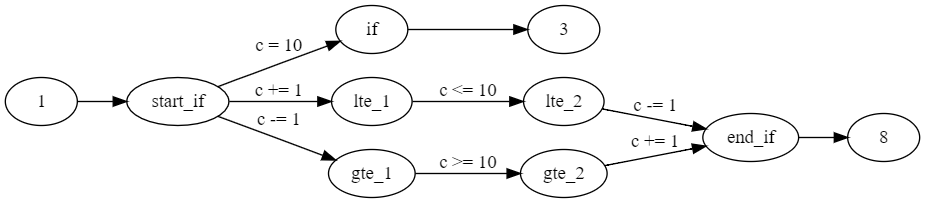
\includegraphics[width=\linewidth]{inequality_expression}
	\caption{Example of an inequality expression.}
	\label{fig:inequality_expression}
\end{figure}

The first transition chain follows the \textit{lte} nodes, which starts with \textit{c += 1} followed by \textit{c \textless =10}, followed by \textit{c -= 1}, which results in the same expression as saying the original counter is strictly smaller than 10. The final \textit{c -= 1} is there to reset the counter, so that the counter is back to what it originally was. 

The second transition chain follows the \textit{gte} nodes, with the first transition being \textit{c -= 1}, followed by \textit{c \textgreater =10}, followed by \textit{c += 1}. This chain states that the counter must be strictly greater than 10.

If either of these can be taken, we can state that the counter must be different to the compared value (in this case 10), as these both express a strict inequality. 

\subsubsection{Less than and greater than}
\label{sec:strict}
The final addition to the set of supported statements, are the less than and greater than expressions. These are needed to model the opposing conditions to greater than or equal and less than or equal respectively.

\begin{lstlisting}[style=CStyle]
bool is_ten(int c){
	if(c <= 10){
		if(c < 10){
			return false;
		}
		return true;
	}
	return false;
}
\end{lstlisting}

The is\_ten code segment models both a less than or equal condition and a less than condition. The first condition will need to be opposed with a strictly greater than condition, and the second one with a greater than or equal condition.

\begin{figure}[h]
	\centering
	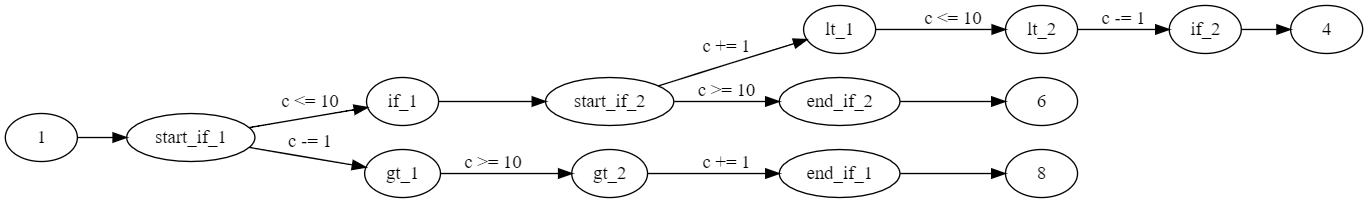
\includegraphics[width=\linewidth]{less_than_greater_than}
	\caption{Example of a less than expression and a greater than expression.}
	\label{fig:less_than_greater_than}
\end{figure}

A simplified version of the counter automaton of the is\_ten function can be seen in Figure \ref{fig:less_than_greater_than}. This automaton has \textit{start\_if\_1} as the start of the outer if and it has \textit{if\_1} and \textit{end\_if\_1} as respective if and end nodes. The inner if has \textit{start\_if\_2} as the start node, \textit{if\_2} as the start of the if segment, and \textit{end\_if\_2} as the end node.

The strict greater than condition, originating from node \textit{start\_if\_1} and ending in node \textit{end\_if\_1}, consists of 3 different transitions. The first transitions \textit{c -= 1} and \textit{c \textgreater =10}, test if the counter is strictly greater. The third transition \textit{c += 1} is there to make sure that the counter goes back to its original value.

The strict less than condition, originating from node \textit{start\_if\_2} and ending in node \textit{if\_2}, consists of \textit{c += 1} and \textit{c \textless =a} as their first two transitions, which can only be satisfied in case the counter is strictly less than a. The final condition \textit{c -= 1} is there to make sure the counter goes back to its original value.

\subsubsection{Iteration statements}
We will also need the notion of iteration statements, which needs 5 additional special nodes to fully support it's functionality. The first node will be the \textit{start of the loop}. The second node is the \textit{pre node}, this node symbolizes the state after the precondition of the for loop has been evaluated. Next we need a node to identify the \textit{start of the inner segment}, which will be reached by a transition with the condition as a label. 

After this node the inner segment will follow, and it will be finalized with the \textit{stop inner segment} node, in case this one is needed. This stop node will symbolize the state after the post expression of the for loop has been evaluated, after this node, a transition will occur to the pre node, to re-evaluate the loop condition.

Finally, one more node is needed, and this node will symbolize the \textit{end of the loop}. This node will always be the last node that gets generated, so that any nodes generated beyond this point will start from this point.

Consider the following segment of code, this will result in the automaton in Figure \ref{fig:test_counter_automaton}.
\begin{lstlisting}[style=CStyle]
bool test(int c){
	for(c = 0; c < 5; c ++){
		continue;
	}
	return true;
}
\end{lstlisting}

\begin{figure}[h]
	\centering
	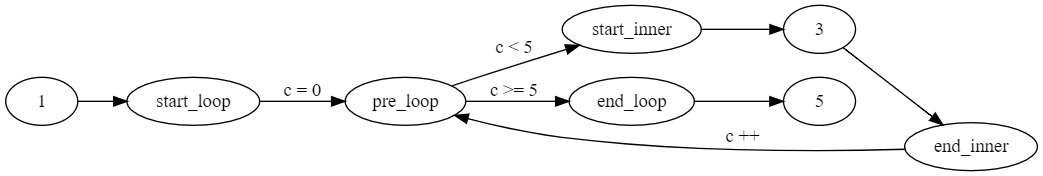
\includegraphics[width=0.95\linewidth]{test_counter_automaton}
	\caption{Example of an Iteration Statement.}
	\label{fig:test_counter_automaton}
\end{figure}

\subsubsection{If statements}
\label{sec:if}
Another important construct are the if statements. These statements will, just as the iteration statements did, require additional nodes to be able to be modelled. If statements require a total of 4 nodes to be modelled.

First of all, we need a $start\ if$ node, from which the conditions will start.

We will need an $if$ node and an $else$ node which will both signify the start of the if and possible else segment.

After the inner segment, they will all end up at the $end\ if$ node from which point they will continue with the next line of code.

Consider the test2 function, and the corresponding simplified counter automaton.
\begin{lstlisting}[style=CStyle]
bool test2(int c){
	if(c == 1){
		printf("The counter is equal to 1.");
	}
	else if(c == 2){
		printf("The counter is equal to 2.");
	}
	return true;
}
\end{lstlisting}

\begin{figure}[h]
	\centering
	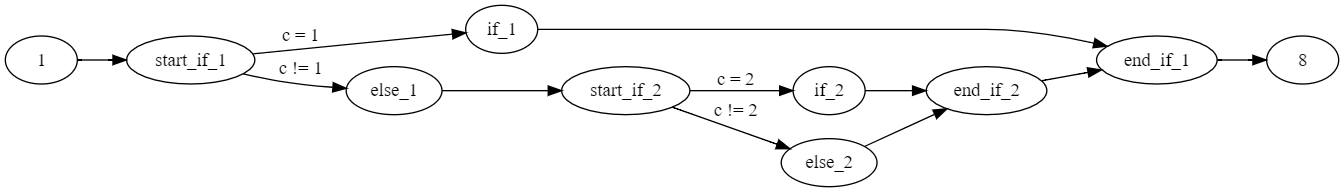
\includegraphics[width=\linewidth]{test2_counter_automaton}
	\caption{Example of if statements.}
	\label{fig:test2_counter_automaton}
\end{figure}

The program will return a more in depth version of the simplified counter automaton displayed in Figure \ref{fig:test2_counter_automaton}. The first if statement will start from $start\_if\_1$, and end at $end\_if\_1$, the else if will start from $start\_if\_2$, and end at $end\_if\_2$.

\subsubsection{Switch statements}
A second conditional statement that exists in c, is a \textit{switch statement}. This statement allows a variable to be compared against multiple values. What is special about the switch statements, is that if matched with one case, the code of all consequential cases will also be executed, until the end of the switch, or until a jump occurs.

Consider the following code snippet. In this case, a variable a will be compared with multiple values, and depending on the matched case, a number of prints will occur.

\begin{lstlisting}[style=CStyle]
bool test(int a){
	switch(a){
		case 3:
			printf("The parameter is greater than 2.");
		case 2:
			printf("The parameter is greater than 1.");
		default:
			printf("The parameter value is %d", a);
	}
	return true;
}
\end{lstlisting}

To generate a counter automaton for a switch statement, we will start by generating a chain for the statements in the cases. This is represented by the chain starting from \textit{start\_switch}, all the way to \textit{default}, in Figure \ref{fig:counter_switch}.

After that we need to add the conditional branches that correspond to the different cases. A first branch originates from \textit{start\_switch}, and can either go to \textit{case\_3} in case the counter is equal to 3, or to \textit{not\_case\_3} in case the counter is not.

There is a second branch from \textit{not\_case\_3} where we can either go to \textit{case\_2} in case the counter is equal to 2, or to \textit{not\_case\_2} in case the counter is not. Finally, from \textit{not\_case\_2} we will always go to the \textit{default} node.

\begin{figure}[h]
	\centering
	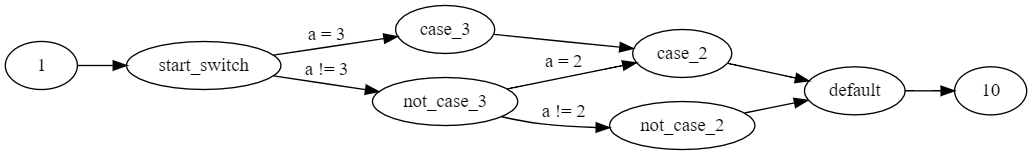
\includegraphics[width=\linewidth]{counter_switch}
	\caption{Example of a switch statement.}
	\label{fig:counter_switch}
\end{figure}

\subsubsection{Counter initialization}
The counters do not get initialized at the point that they got declared within the code. This is a simple improvement that helps to reduce the number of counters. Consider the code segment below, in which two different counters are used.

\begin{lstlisting}[style=CStyle]
bool two_counters(){
	int c = 0;
	int c2 = 0;
	if(c == 2){
		return false;
	}
	else if(c2 == 2){
		return false;
	}
	return true;
}
\end{lstlisting}
The first counter will be initialized just before the if statement gets used. The second counter will not be initialized at that point, but will only be initialized just before the second if statement gets used. This means that the program will in fact be able to support the given code segment, even though it has two different counters.

\subsubsection{Final overview}
To give a in depth overview of how the conversion works, we will transform the following code into a counter automaton. This code consists of multiple if statements, as well as a loop, it makes use of a single counter value, being \textit{counter}, and two parameters. The loop and the final \textit{if} both use inequality expressions, which are representable in a counter automaton, as was described earlier. The first two \textit{ifs} make use of relational expressions with the $<$ and $>$ operators, which are also representable within a counter automaton. The counter is only  using additions or subtractions with parameters and none of these parameters will ever be modified, which also conforms to the requirements. Finally, this function has only integer parameters and a bool return type, which makes us conclude that this entire function is representable in a counter automaton.

\begin{lstlisting}[style=CStyle]
bool gcm(int a, int b){
	int counter = a;
	counter -= b;
	int i1 = 1;
	int i2 = 1;
	while(counter != 0){
		if(counter > 0){
			counter -= b;
			i2 += 1;
		}
		else if(counter < 0){
			counter += a;
			i1 += 1;
		}
		if(counter == 0){
			printf("the greatest multiple is equal to ");
			printf("%d * %d = %d * %d = %d.", i1, a, i2, b, i1*a);
		}
	}
	return true;
}
\end{lstlisting}

The first line is the function definition, this will just be converted to a node with label 1, representing the first line. Since this is the first node added to the counter automaton, it will also be denoted as being the initial node, as can be seen in Figure \ref{fig:final_overview_1}

\begin{figure}[h]
	\centering
	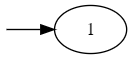
\includegraphics[width=0.2\linewidth]{final_overview_1}
	\caption{First node in the counter automaton.}
	\label{fig:final_overview_1}
\end{figure}

The second line is of interest to the counter machine, as it is a counter modification. However it will not directly generate any special counter automaton configuration, as declarations of counters are only displayed as soon as a counter is actually used or modified. Since nothing special is generated, it will simply generate a new node representing the current line (being 2), with a transition coming from the last added node before this one, as displayed in Figure \ref{fig:final_overview_2}.

\begin{figure}[h]
	\centering
	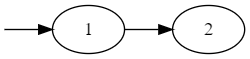
\includegraphics[width=0.4\linewidth]{final_overview_2}
	\caption{Automaton corresponding to the second line of \textit{gcm}.}
	\label{fig:final_overview_2}
\end{figure}

\newpage

The third line is an actual modification to the counter, so before we generate any additional nodes regarding the operation specified on this line, we need to add the counter initialization as a \textit{pre} statement for this line, this is represented by the tool by decrementing the current line in steps of 0.01. An assignment operation requires three additional nodes, so we will make use of the nodes 2.97, 2.98 and 2.99 to model the assignment functionality, as visualised in Figure \ref{fig:final_overview_3}.

\begin{figure}[h]
	\centering
	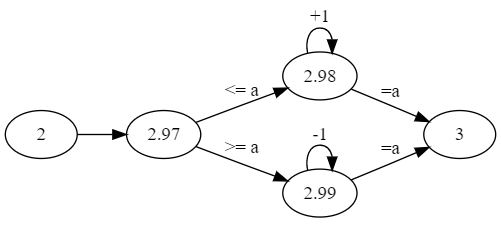
\includegraphics[width=0.7\linewidth]{final_overview_3}
	\caption{Counter automaton modelling the initial assignment of the counter.}
	\label{fig:final_overview_3}
\end{figure}

The actual operation specified on line three, is a subtraction of the counter by the parameter b, as is modelled in the sub counter automaton in Figure \ref{fig:final_overview_4}.

\begin{figure}[h]
	\centering
	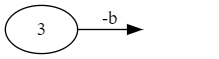
\includegraphics[width=0.35\linewidth]{final_overview_4}
	\caption{Counter automaton modelling the operation on line two.}
	\label{fig:final_overview_4}
\end{figure}

Line four and five are both statements that are not of relevance to the counter, and will therefore be simply represented as a sequential chain following from the last added node, being node 3, as can be seen in Figure \ref{fig:final_overview_5}.

\begin{figure}[h]
	\centering
	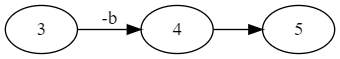
\includegraphics[width=0.5\linewidth]{final_overview_5}
	\caption{Counter automaton resulting from line four and five.}
	\label{fig:final_overview_5}
\end{figure}

The sixth line defines a while loop. This requires us to add several nodes that are all related to the statement on line six. The tool will symbolise this by incrementing the current line in steps of 0.01. So 4.01 is a node that is used to help model a statement on line four.

First we need two nodes, one symbolising the start of the inner branch, modelled by the node with label 6.02, and one the symbolise the end of the loop, modelled by the node with label 6.01.

The loop ends as soon as the while condition no longer holds, and therefore the transition from start node, 6, to the end of the loop, 6.01 is a condition checking whether or not the condition of the while loop no longer holds, in this case this condition is represented as equality to zero, being the opposite condition to inequality to zero. 

The loop continues as long as the condition holds, which is modelled by the sequence going from the start node, 6.01, to the start of the inner loop, being 6.02. This configuration models an inequality to zero expression, as described in Section \ref{sec:inequality}, \nameref{sec:inequality}.

\begin{figure}[h]
	\centering
	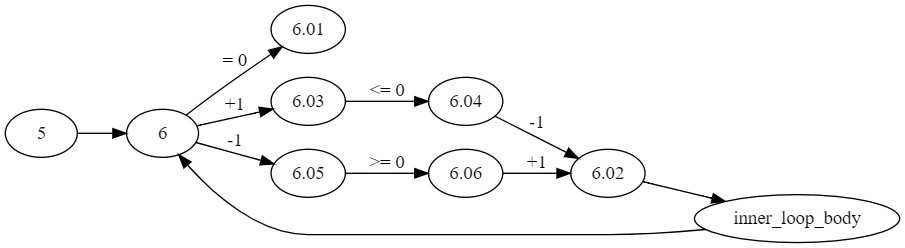
\includegraphics[width=\linewidth]{final_overview_6}
	\caption{Counter automaton resulting from line six.}
	\label{fig:final_overview_6}
\end{figure}

Lines seven until ten define the first selection statement. Selection statements require, as referenced in Section \ref{sec:if}, \nameref{sec:if}, three additional nodes to fully model the needed implementation.

The start of the selection statement, is modelled by the node with label 7. From this node, there is a transition going to the node with label 7.03, which symbolises the else branch, and therefore the transition to this node symbolises all counter values for which the if condition would not hold, which in this case are all counters smaller than or equal to zero.

The second transition originating from the start of the selection statement symbolises the cases where the counter satisfies the selection condition. The node 7.01 symbolises the start of the inner body of the if statement. The chain of transitions starting from 7 and going to node 7.01 model strict greater than, as is explained in Section \ref{sec:strict}, \nameref{sec:strict}.

Finally, there is the \textit{end of if statement} node, being node 7.02. This node symbolises the end of all branches, so if there were any else branches, they will also end in this node.

The inner body is simple and does not need any complex structures to be added. The statement on line 8 will result in a transition originating from node 8 with label $-= b$. The statement on line 9 has no effect on the counter, and will just be modelled with an empty transition.

\begin{figure}[h]
	\centering
	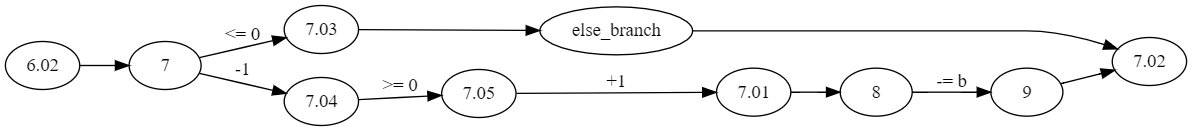
\includegraphics[width=\linewidth]{final_overview_7}
	\caption{Counter automaton resulting from line seven up until line ten.}
	\label{fig:final_overview_7}
\end{figure}

The eleventh until fourteenth line models the else branch of the previous selection statement. This statement follows the same design principles as the previous selection statement did, and will be inserted in the previous counter automaton, in the place where the current \textit{else\_branch} label is, as can be seen in Figure \ref{fig:final_overview_8}. Note that there is no else branch, which was not generated as there are not other \textit{else if} or \textit{else} statements in the code.

\begin{figure}[h]
	\centering
	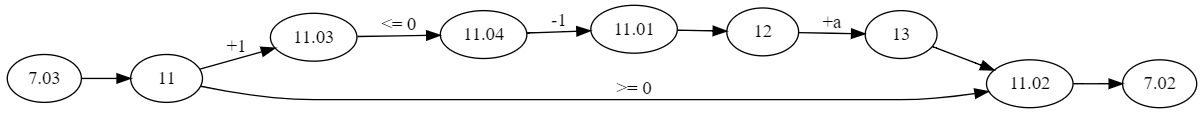
\includegraphics[width=\linewidth]{final_overview_8}
	\caption{Counter automaton resulting from line eleven up until line fourteen.}
	\label{fig:final_overview_8}
\end{figure}

The final selection statement can be found on line fifteen until line eighteen. This statement includes nothing new, and will simply follow the earlier mentioned specification. This selection statement will end with a transition going from the end of the selection, being the node with label 15.02, to the start of the earlier mentioned while statement, being the node with label 6, as can be seen in Figure \ref{fig:final_overview_9}.

\begin{figure}[h]
	\centering
	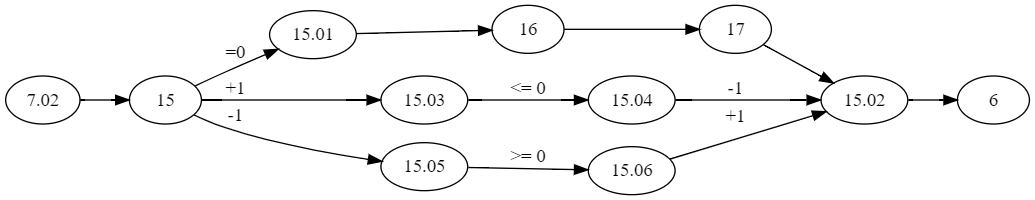
\includegraphics[width=\linewidth]{final_overview_9}
	\caption{Counter automaton resulting from line fifteen up until line eighteen.}
	\label{fig:final_overview_9}
\end{figure}

After this, all that remains is the return on line twenty. This return will simply follow after node 6.01 from the while configuration specified earlier. After a return, no nodes will be generated no matter what the kind of these statement is.

\begin{figure}[h]
	\centering
	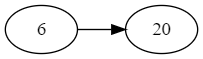
\includegraphics[width=0.35\linewidth]{final_overview_10}
	\caption{Counter automaton modelling the return on line twenty.}
	\label{fig:final_overview_10}
\end{figure}

The complete overview of the counter automaton can be seen in Figure \ref{fig:final_overview_11}. This is a completely correct counter automaton that is suitable for reachability analysis.

\begin{landscape}
	\begin{figure}
		\centering
		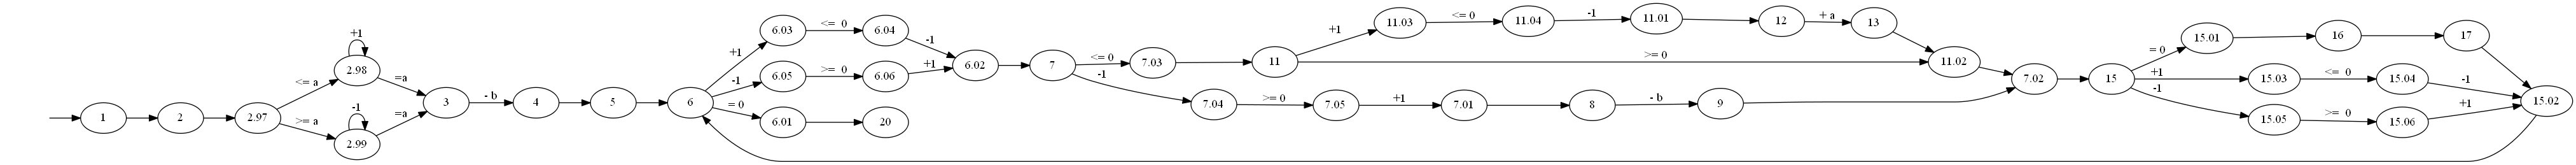
\includegraphics[width=\linewidth]{final_overview_11}
		\caption{Counter automaton modelling the return on line twenty.}
		\label{fig:final_overview_11}
	\end{figure}
\end{landscape}

\section{Tool Validation}
To determine the corectness of our tool, we created a test suite consisting out of three groups of tests, which are all white box tests. The tests will check the outputted dot and the trace output of the program, against traces and dot files which have been manually generated and verified.

The first group will only test the first loop of the program, and it will check whether or not all nodes get properly generated. This purely tests on the generation of nodes, and will not regard any variation in configuration in which these nodes could occur.

The second group will test the cleaner. It will test most cases (all common cases) in which folding and substituting should occur as well as the cases where it should not fold anything. In this group we will also perform extensive symbol table testing, to check whether or not all values get properly tracked by the symbol table.

The third group will test the full tool. It will validate the dot file resulting from the cleaner, as well as the dot file(s) resulting from the counter automaton generator. It will also evaluate all output regarding the symbol table, and the potential errors of the code validator. There are happy day tests where each conditional statement gets tested separately, there are tests where conditional statements get nested and there are tests to see whether we can still evaluate conditional statements with constant conditions. Furthermore, there are failure tests that test whether or not we can properly detect incorrect counter types, incorrect parameter types, incorrect number of counters, incorrect conditional operations, incorrect counter modifications and properly detect counters defined in global scopes. There are also tests for edge case scenarios, such as returns in every single branch, the cleaner will not be able to detect these, and therefore the generator should be able to stop generating all nodes, once there are no branch that can carry on.

The test coverage was validated using Codecov, which gave a total line coverage of 93\% at the end of development. This coverage was used as a metric to determine whether or not there were sufficient tests at each stage of development. The remaining 7\% are trivial lines that did not need any testing, such as \textit{\_\_str\_\_} operators.

\section{Conclusion}
In this paper we propose an algorithm for converting a small subset of the c language to counter automata, and discuss its implementation. The resulting automata can be used in reachability analysis within the code. 

The paper gives a description on all the steps the program goes through in order to achieve this counter automaton, as well as a brief insight in why things are the way they are.

This proposed algorithm can be used to improve existing static code analysis and will furthermore be usable to solve the halting problem for a subset of c programs. It is however only usable in a limited amount of cases, in more complex situations, where reachability analysis would be far more desired, it will most likely not be usable as chances of violated conditions will be high. In the situations where it is applicable, big conditional statements or a large amount of conditional statements can make determining the reachability of certain sub segments hard, and with the addition of this algorithm as a reachability checker, it could definitely lead to improvements in coding.

\section{Future work}
One of the future aspects that still needs to be worked on, is the precision, efficiency and usefulness of the program. The program is too restrictive to be practically usable, and should therefore be expanded to support further c code.

Furthermore, before the resulting counter automata have any use, there needs to be an expansion to the tool, which will allow the evaluation of counter automata, so that actual reachability conclusions can be made.
\printbibliography
\end{document}